\newpage
\section{$\Hww$ tagger limits (categories Hww1, Hww2, Hww3)}
\label{results}

\iffalse

\begin{figure*}[h!tpb]
\begin{center}
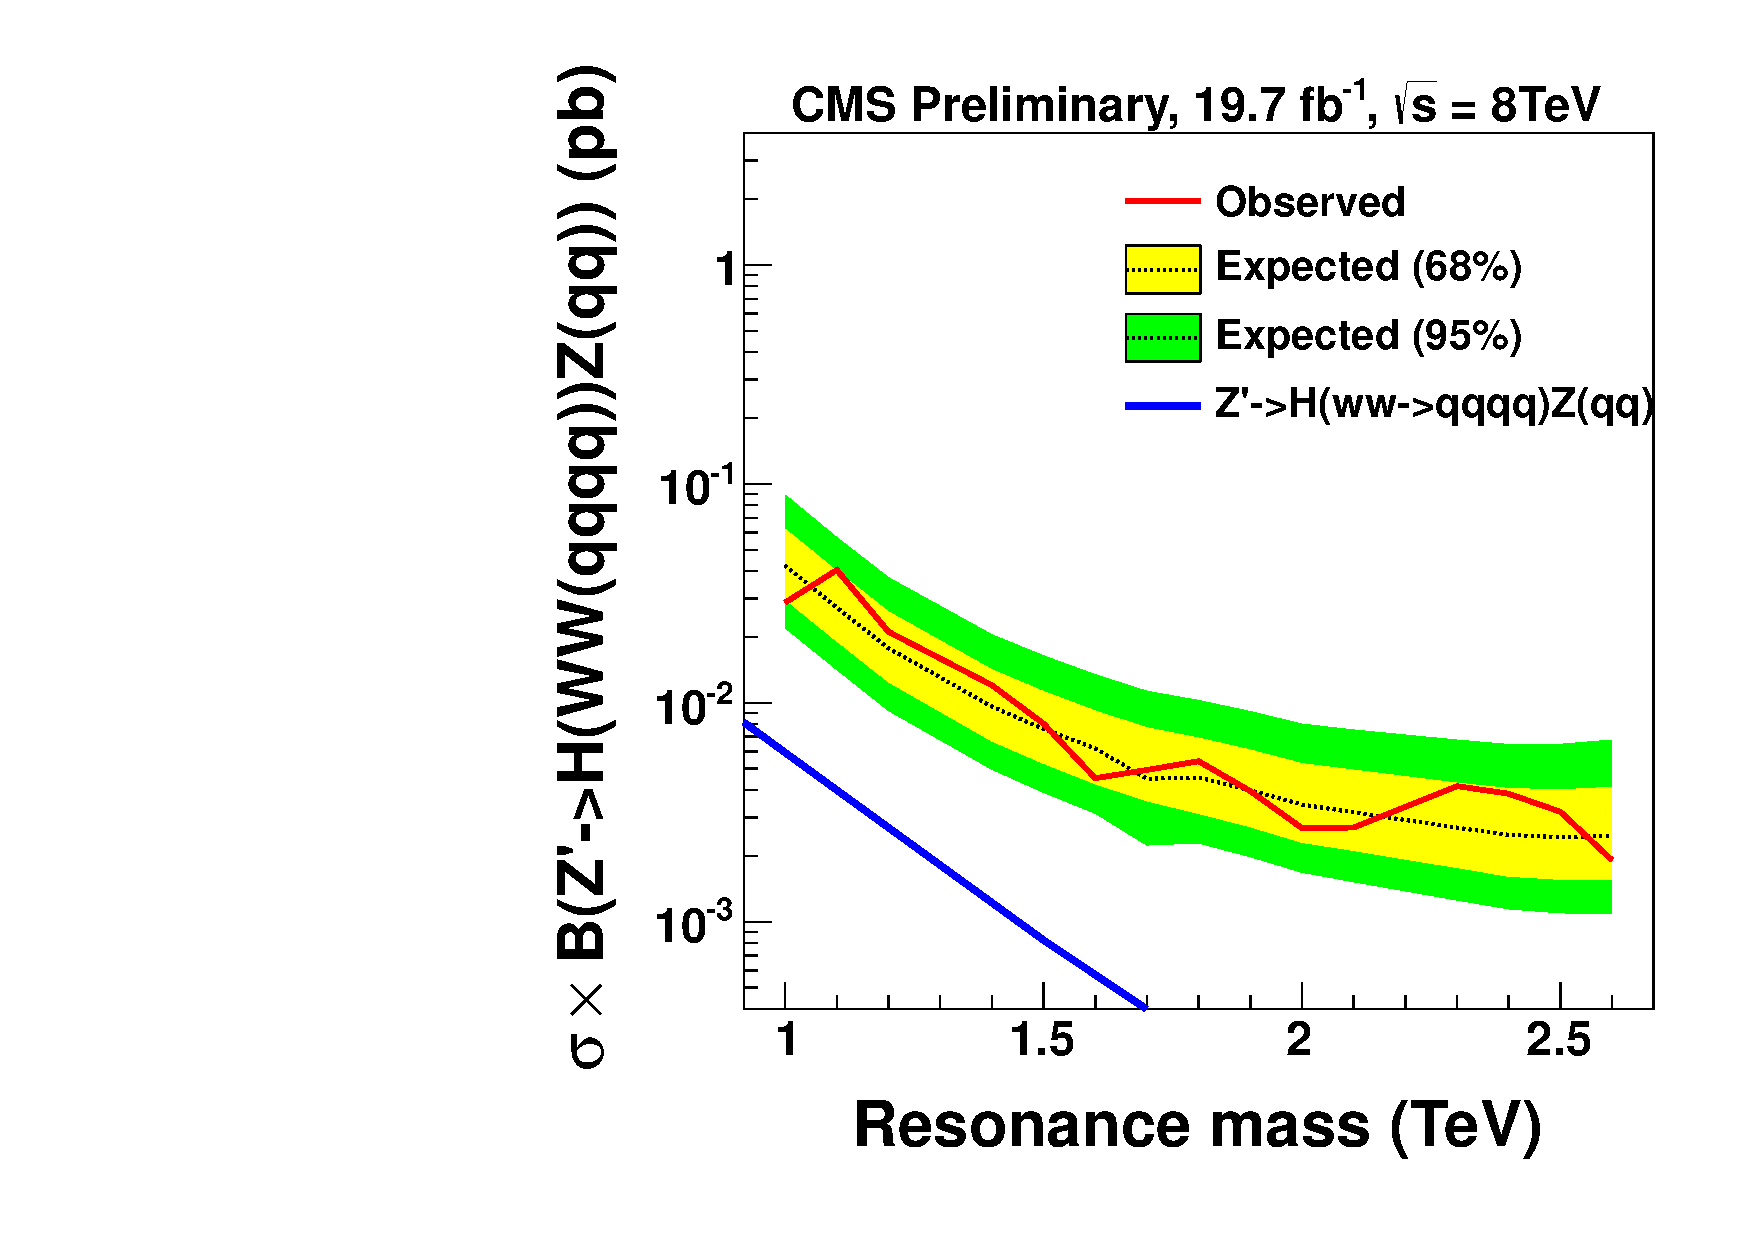
\includegraphics[width=0.49\textwidth]{HqqqqZqqfigs/Limits/brazilianFlag_Hww_Combine.pdf}
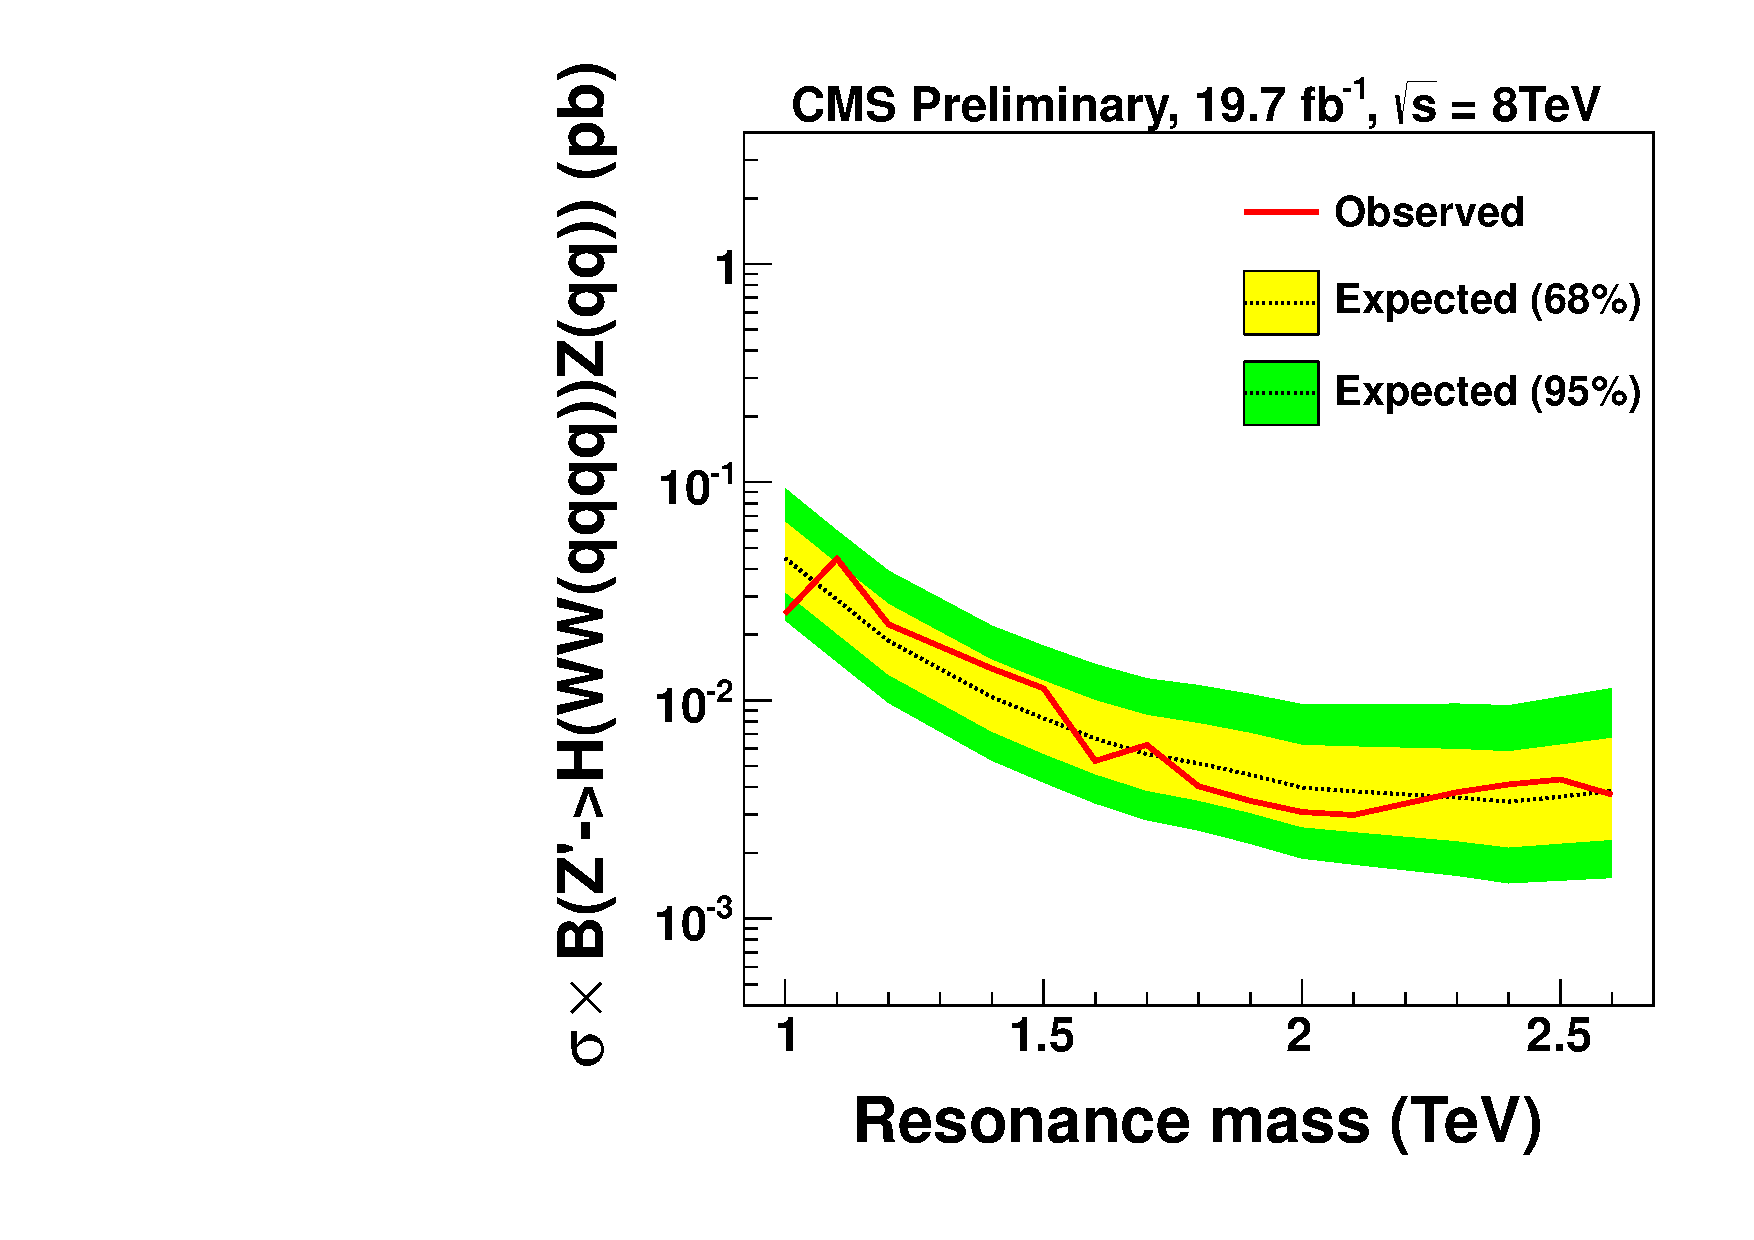
\includegraphics[width=0.49\textwidth]{HqqqqZqqfigs/Limits/brazilianFlag_Hww_.pdf}
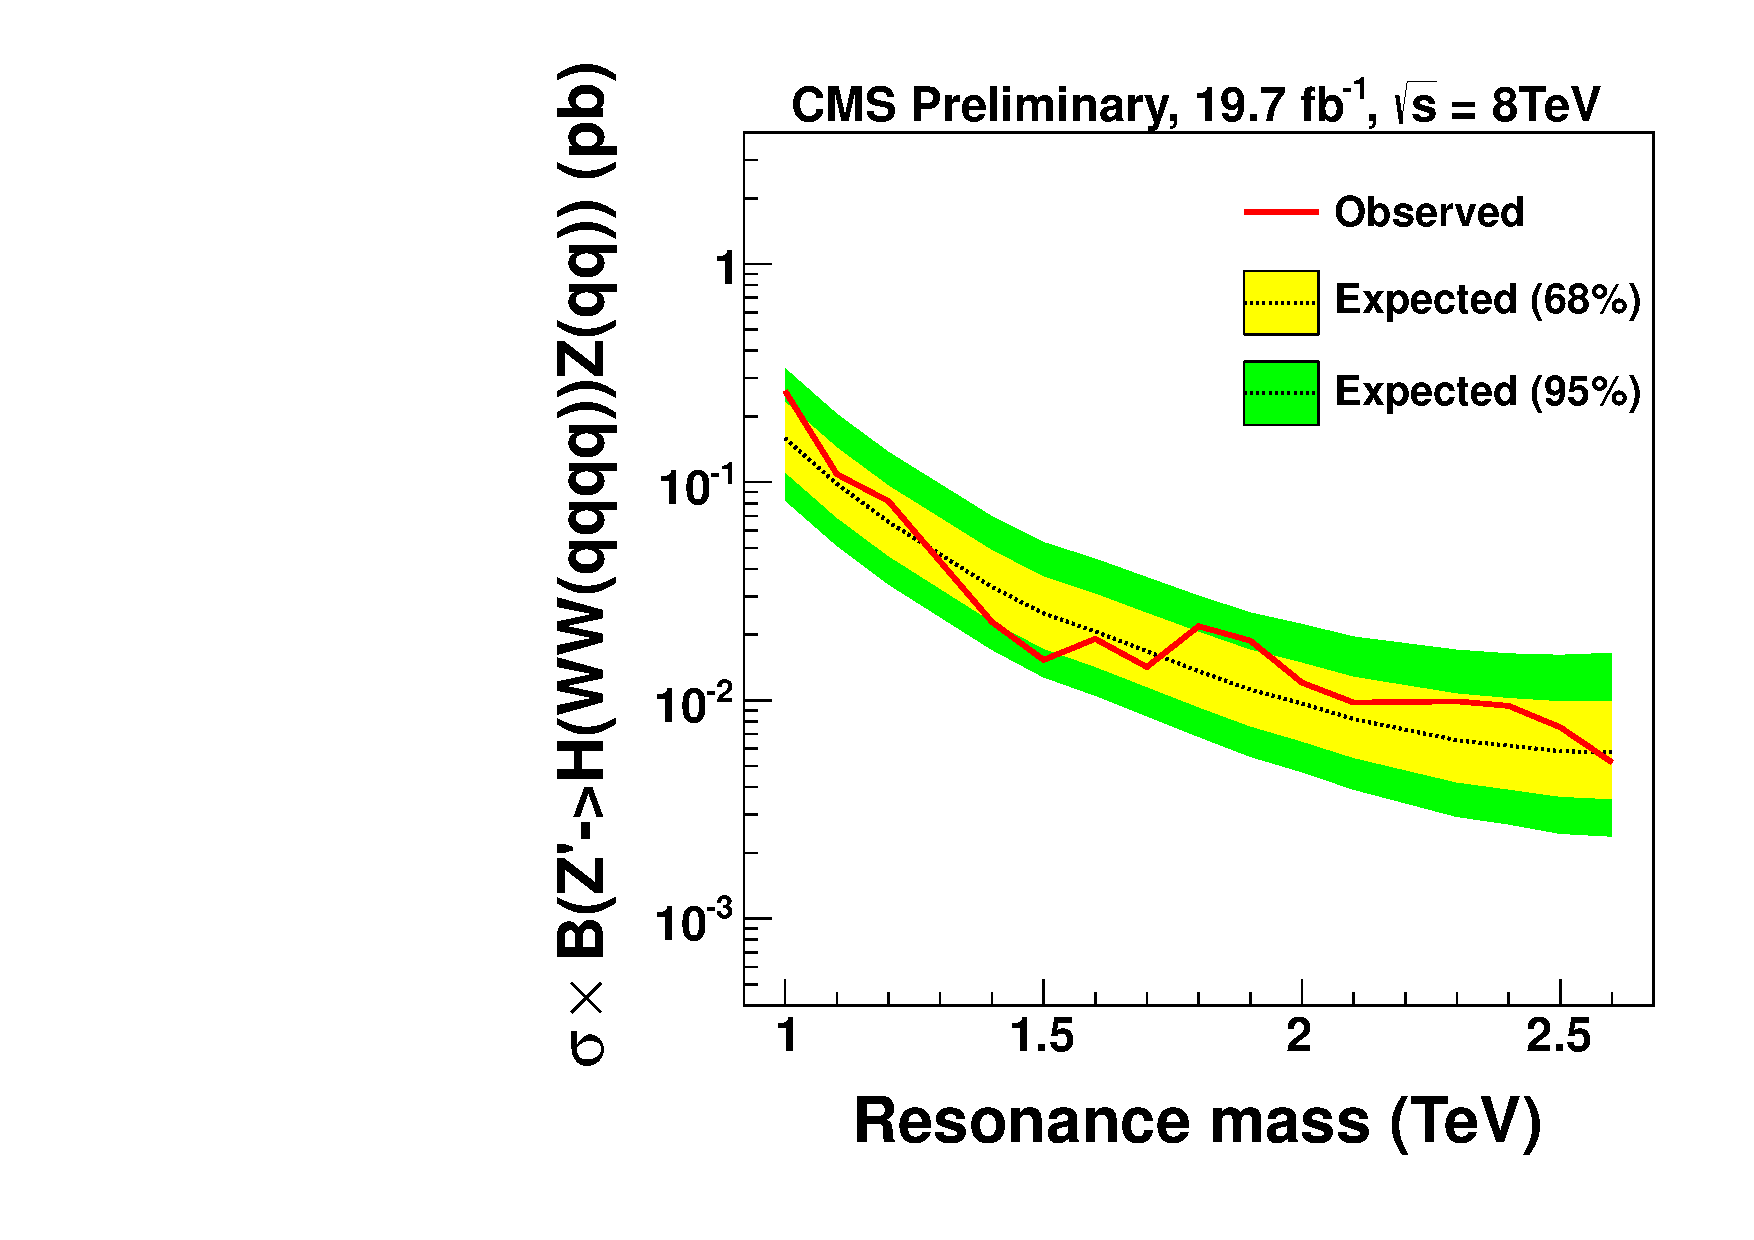
\includegraphics[width=0.49\textwidth]{HqqqqZqqfigs/Limits/brazilianFlag_Hww_LowH.pdf}
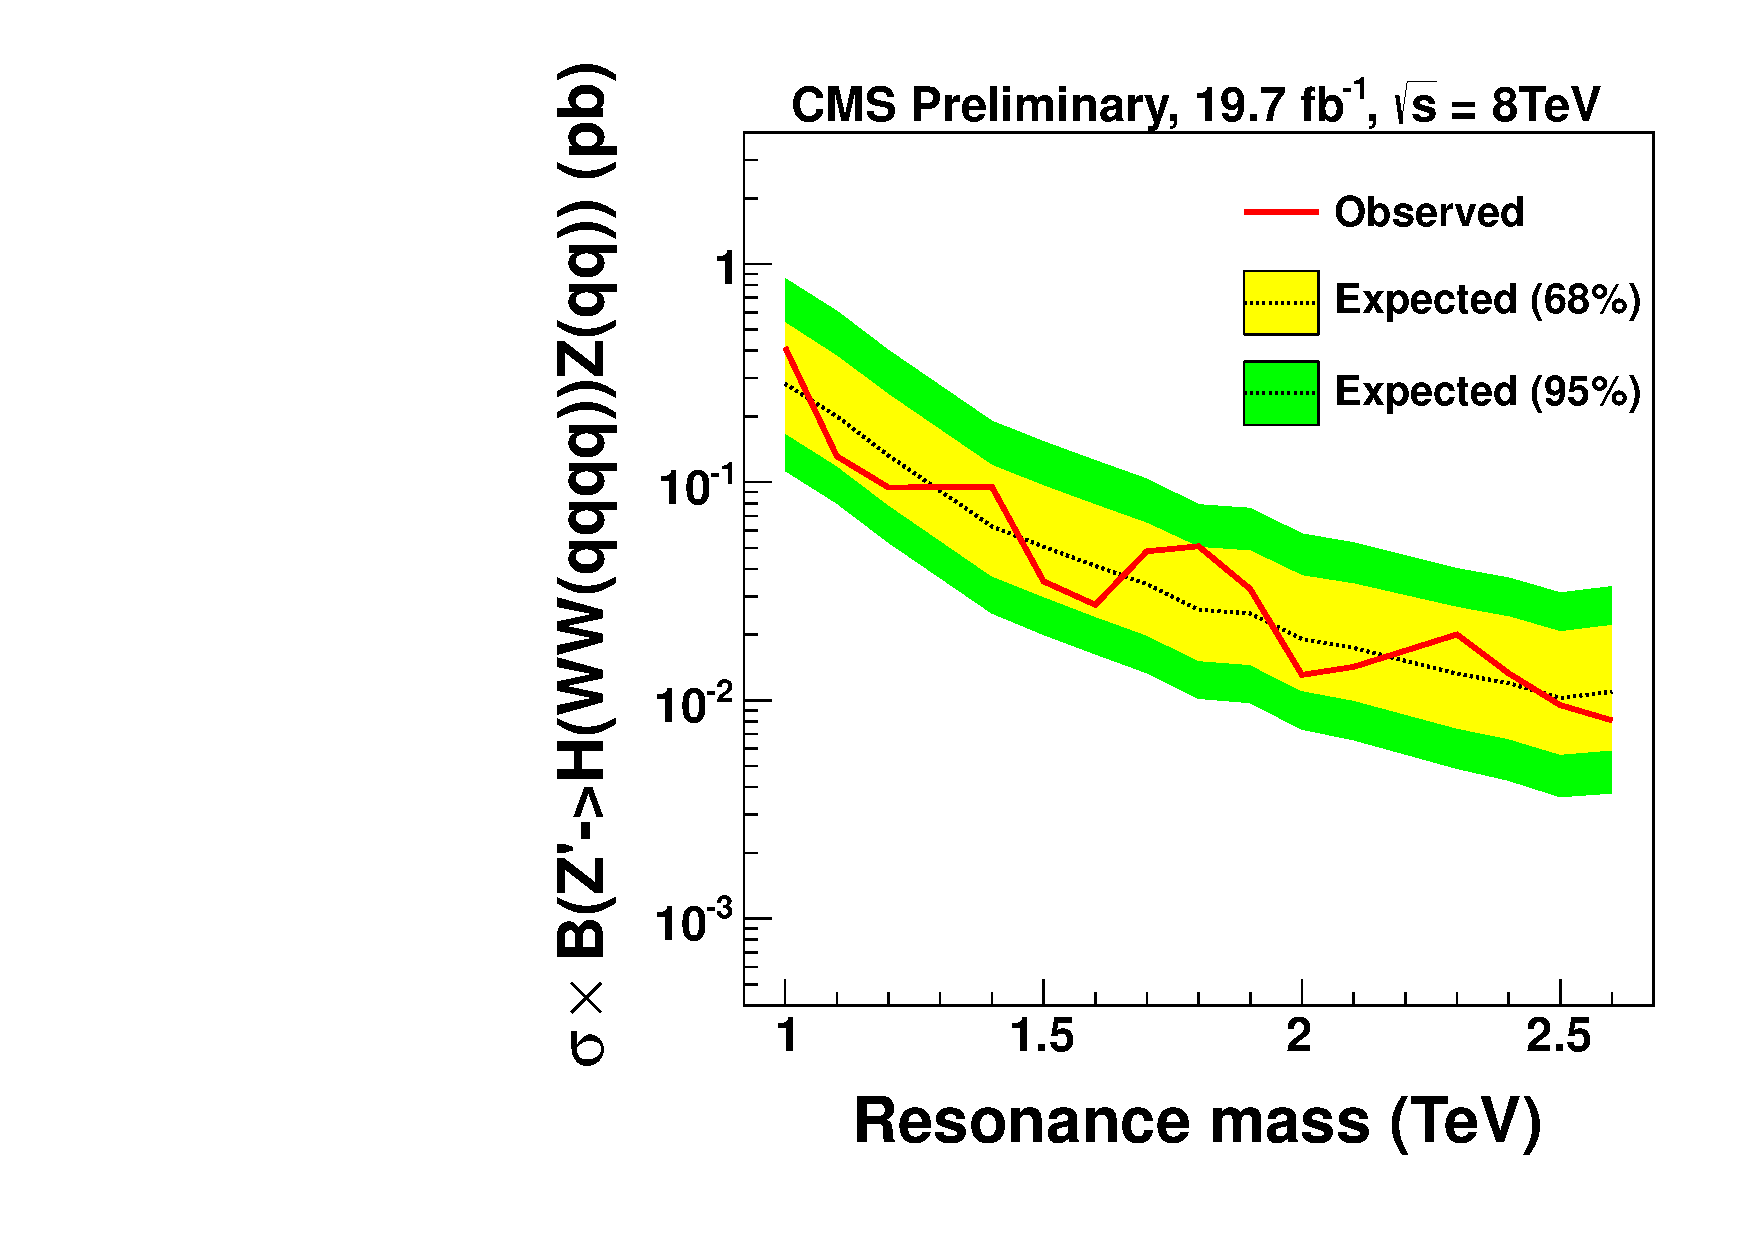
\includegraphics[width=0.49\textwidth]{HqqqqZqqfigs/Limits/brazilianFlag_Hww_LowV.pdf}
\end{center}
\caption{Expected and observed limits for H(ww)Z(qq) search. The combined limit is on top left. the high purity limit
is the top right one. and the low purity H-tagging limit is on the bottom left. the low purity V-tagging on bottom right.   
%  The predicted cross sections as a function of resonance mass for the considered benchmark models are overlaid.
}
\label{fig:HwwZqqLimits}
\end{figure*}

\begin{figure*}[h!tpb]
\begin{center}
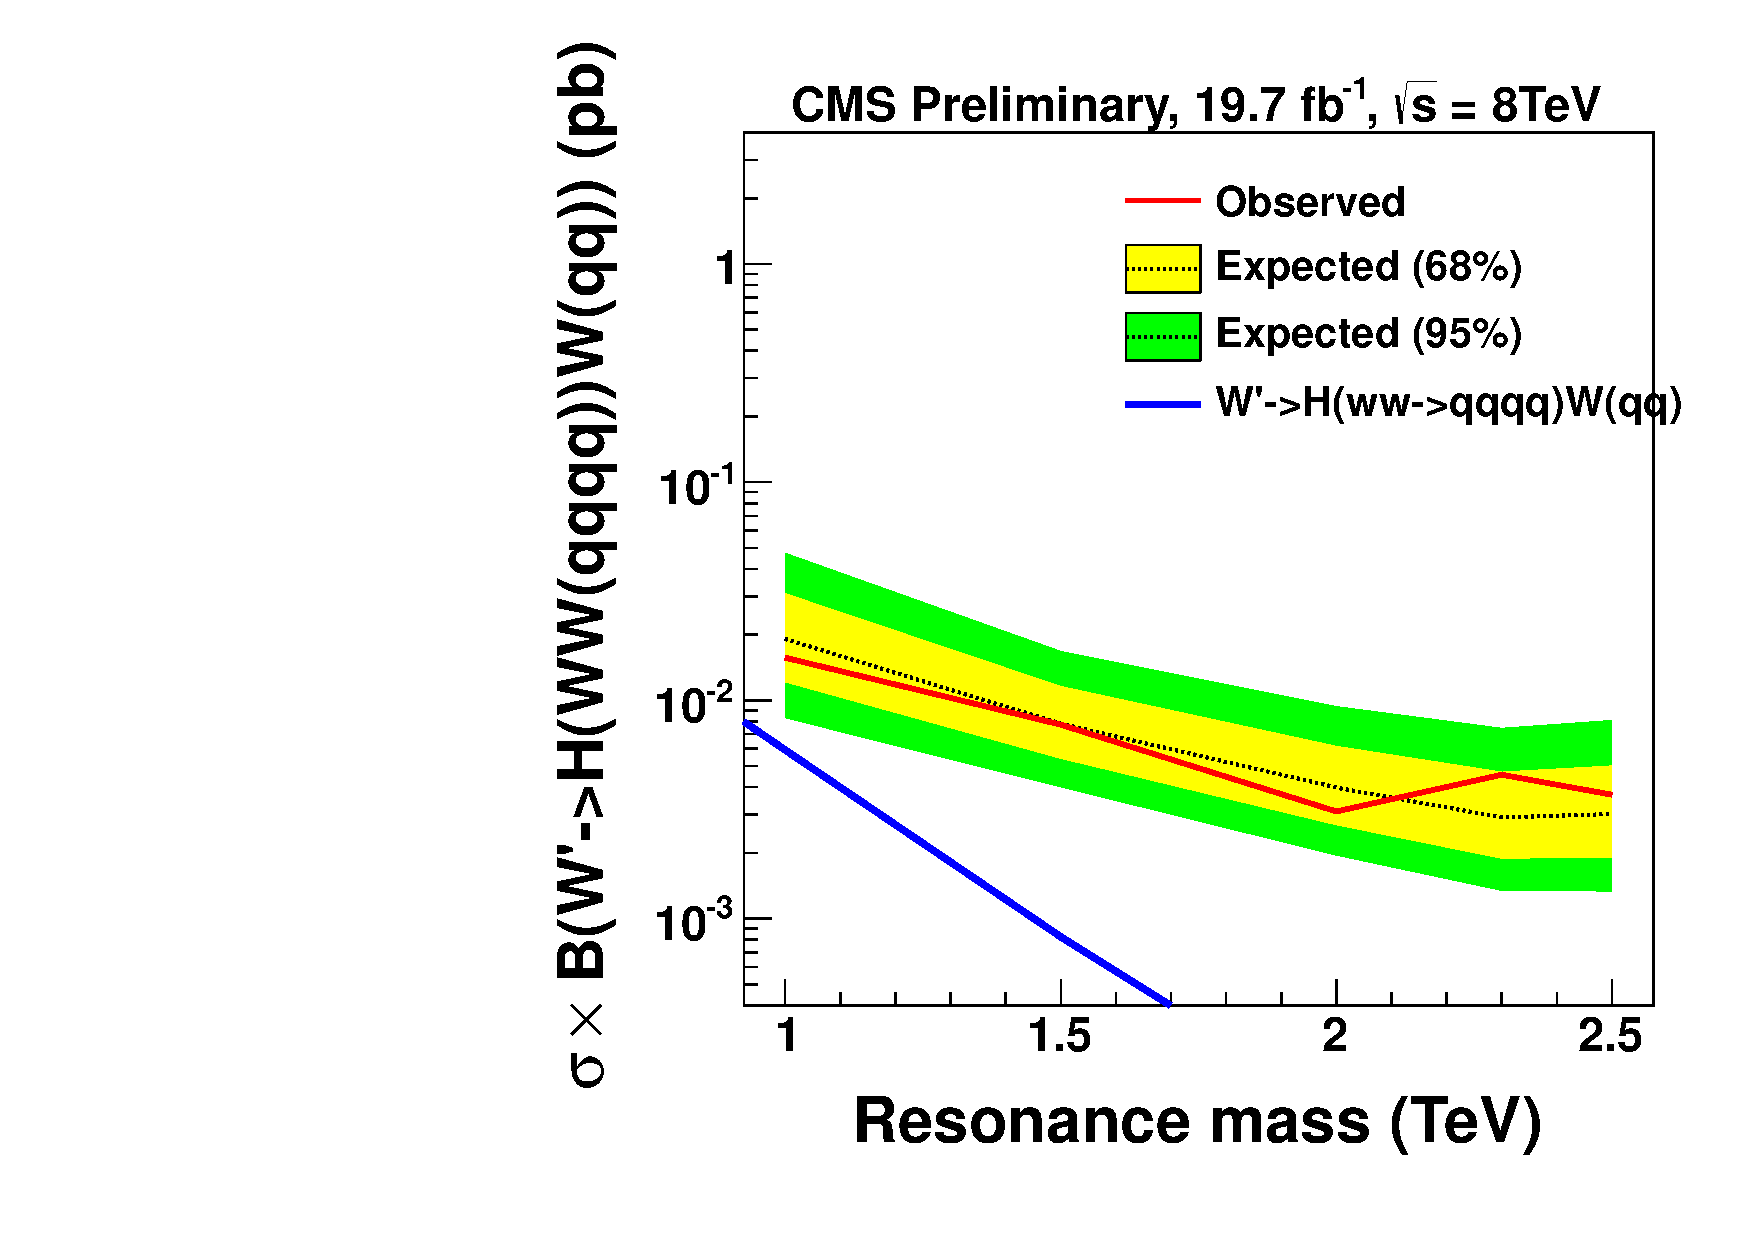
\includegraphics[width=0.49\textwidth]{HqqqqZqqfigs/Limits/brazilianFlag_Hww_HwwWqqCombine.pdf}
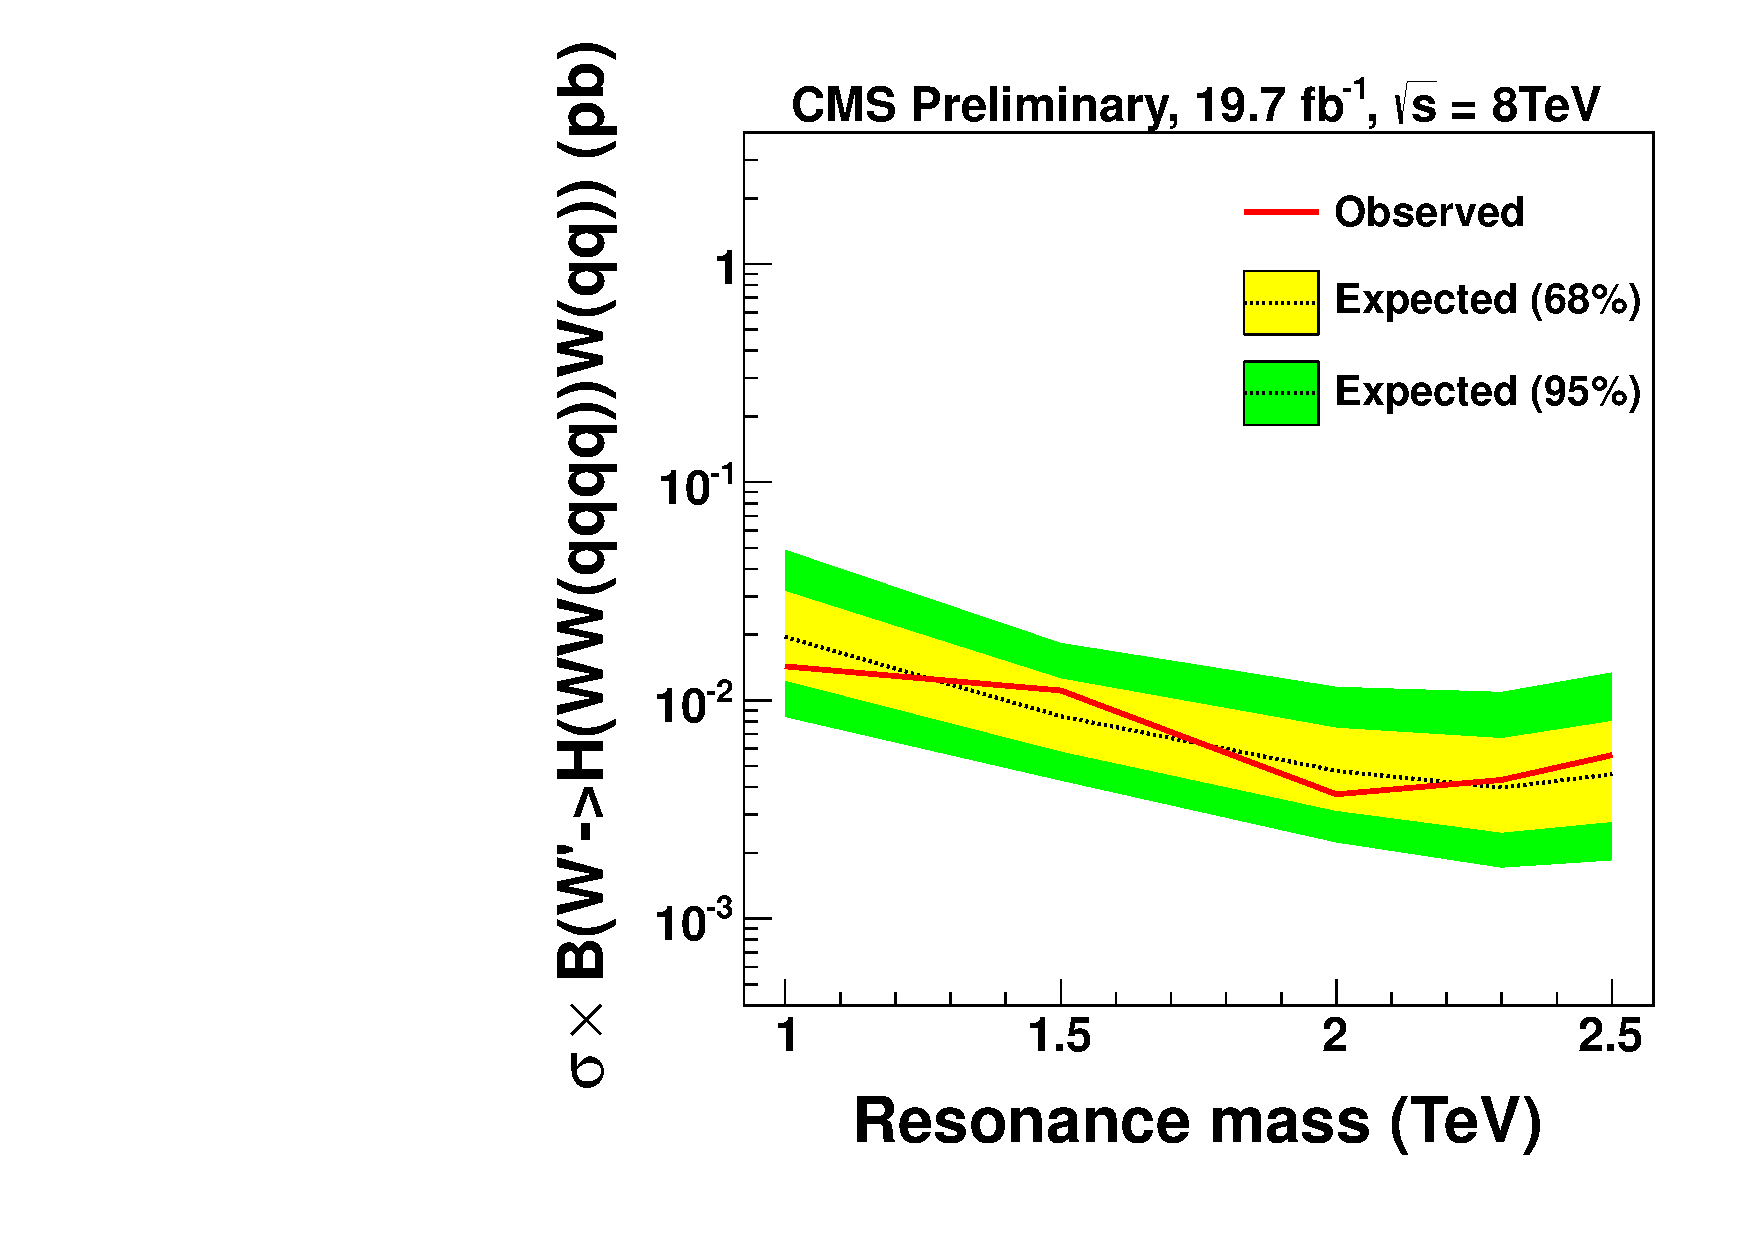
\includegraphics[width=0.49\textwidth]{HqqqqZqqfigs/Limits/brazilianFlag_Hww_HwwWqq.pdf}
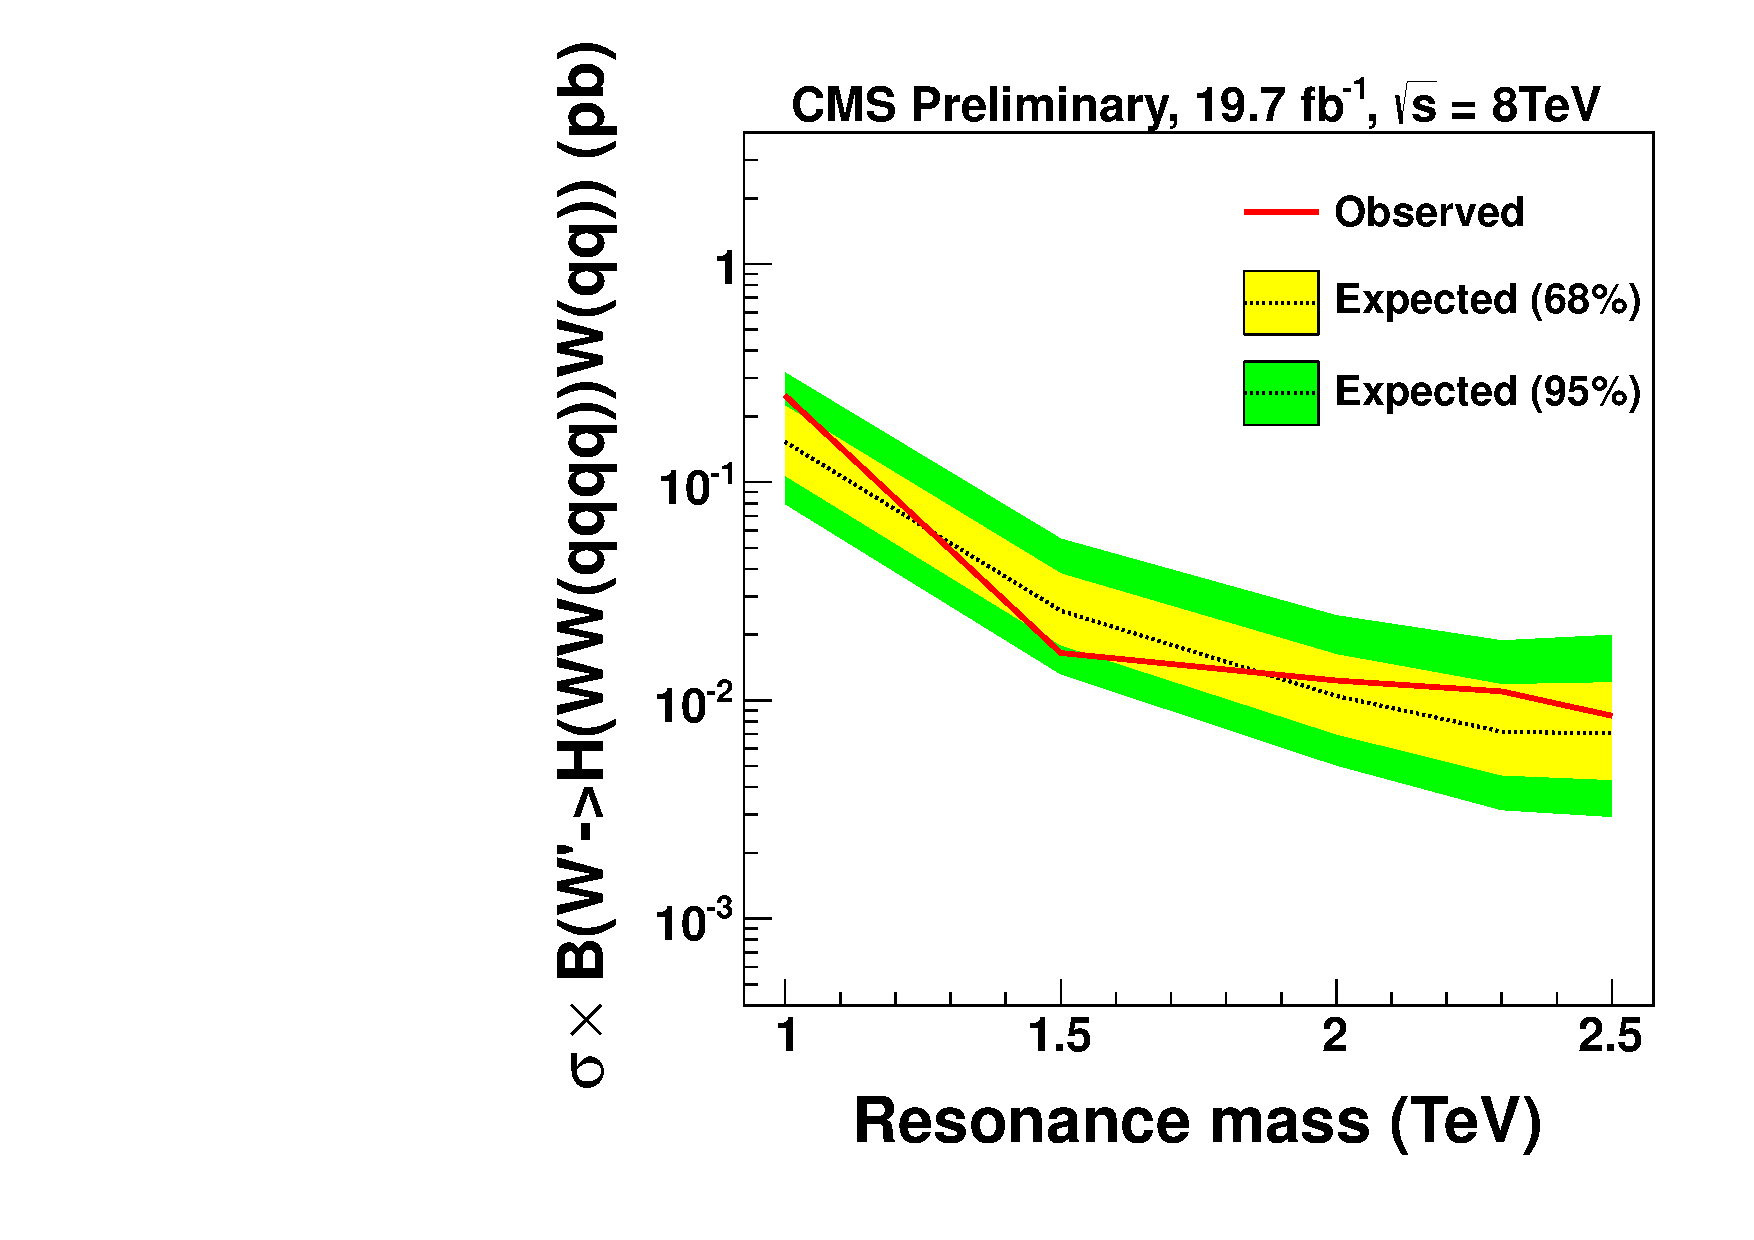
\includegraphics[width=0.49\textwidth]{HqqqqZqqfigs/Limits/brazilianFlag_Hww_HwwWqqLowH.pdf}
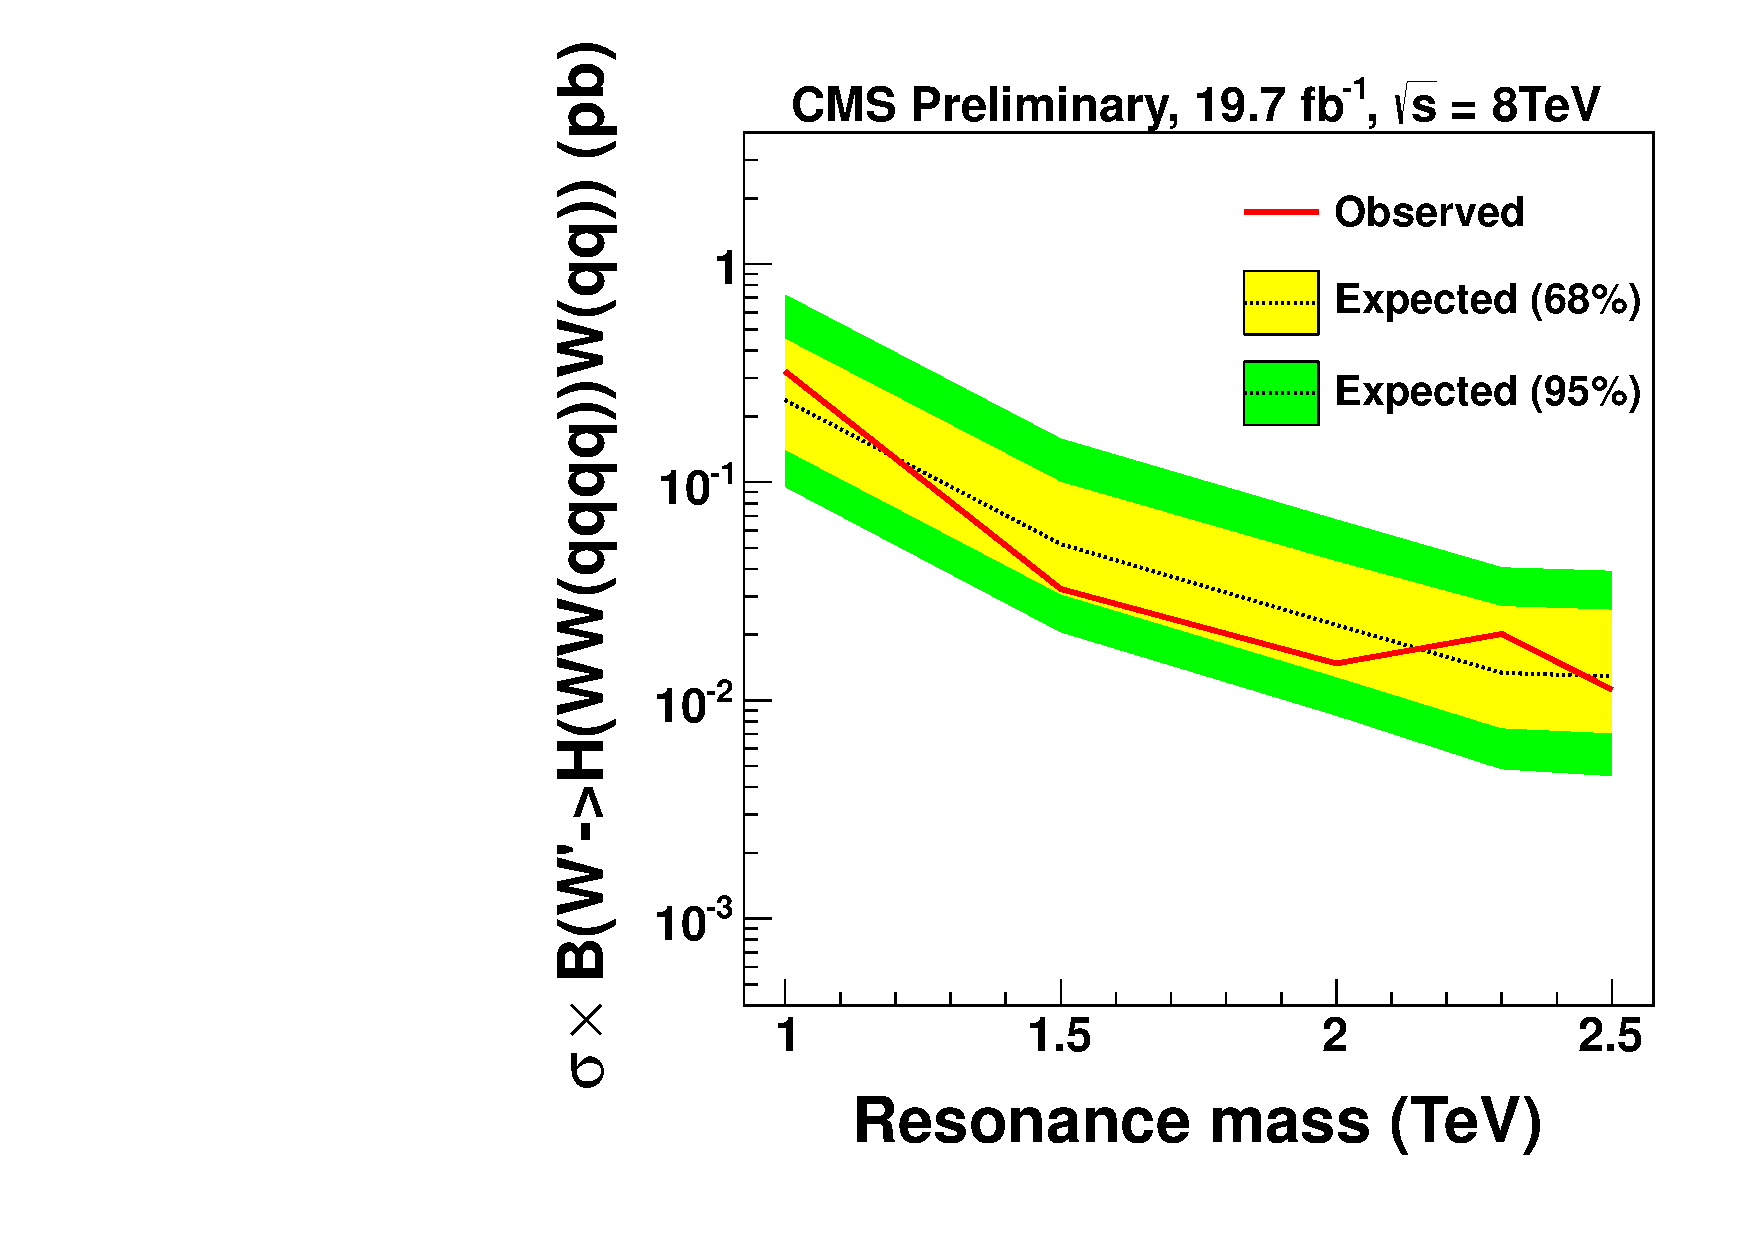
\includegraphics[width=0.49\textwidth]{HqqqqZqqfigs/Limits/brazilianFlag_Hww_HwwWqqLowV.pdf}
\end{center}
\caption{Expected and observed limits for H(ww)W(qq) search. The combined limit is on top left. the high purity limit
is the top right one. and the low purity H-tagging limit is on the bottom left. the low purity V-tagging on bottom right.   
%  The predicted cross sections as a function of resonance mass for the considered benchmark models are overlaid.
}
\label{fig:HwwWqqLimits}
\end{figure*}

\fi

Figure~\ref{fig:HwwVCombined} shows the cobmined limits for \HwwVqq and \HbbVqq signals failing the 
$\Hbb$ tagger but passing the             
$\Hww$ tagger. Limits of combining category Hww1, Hww2 and Hww3 are presented.
The $\Hww$, $\Hbb$ and V bosons braching ratios are already taken into account.


\begin{figure*}[ht!pb]
\begin{center}
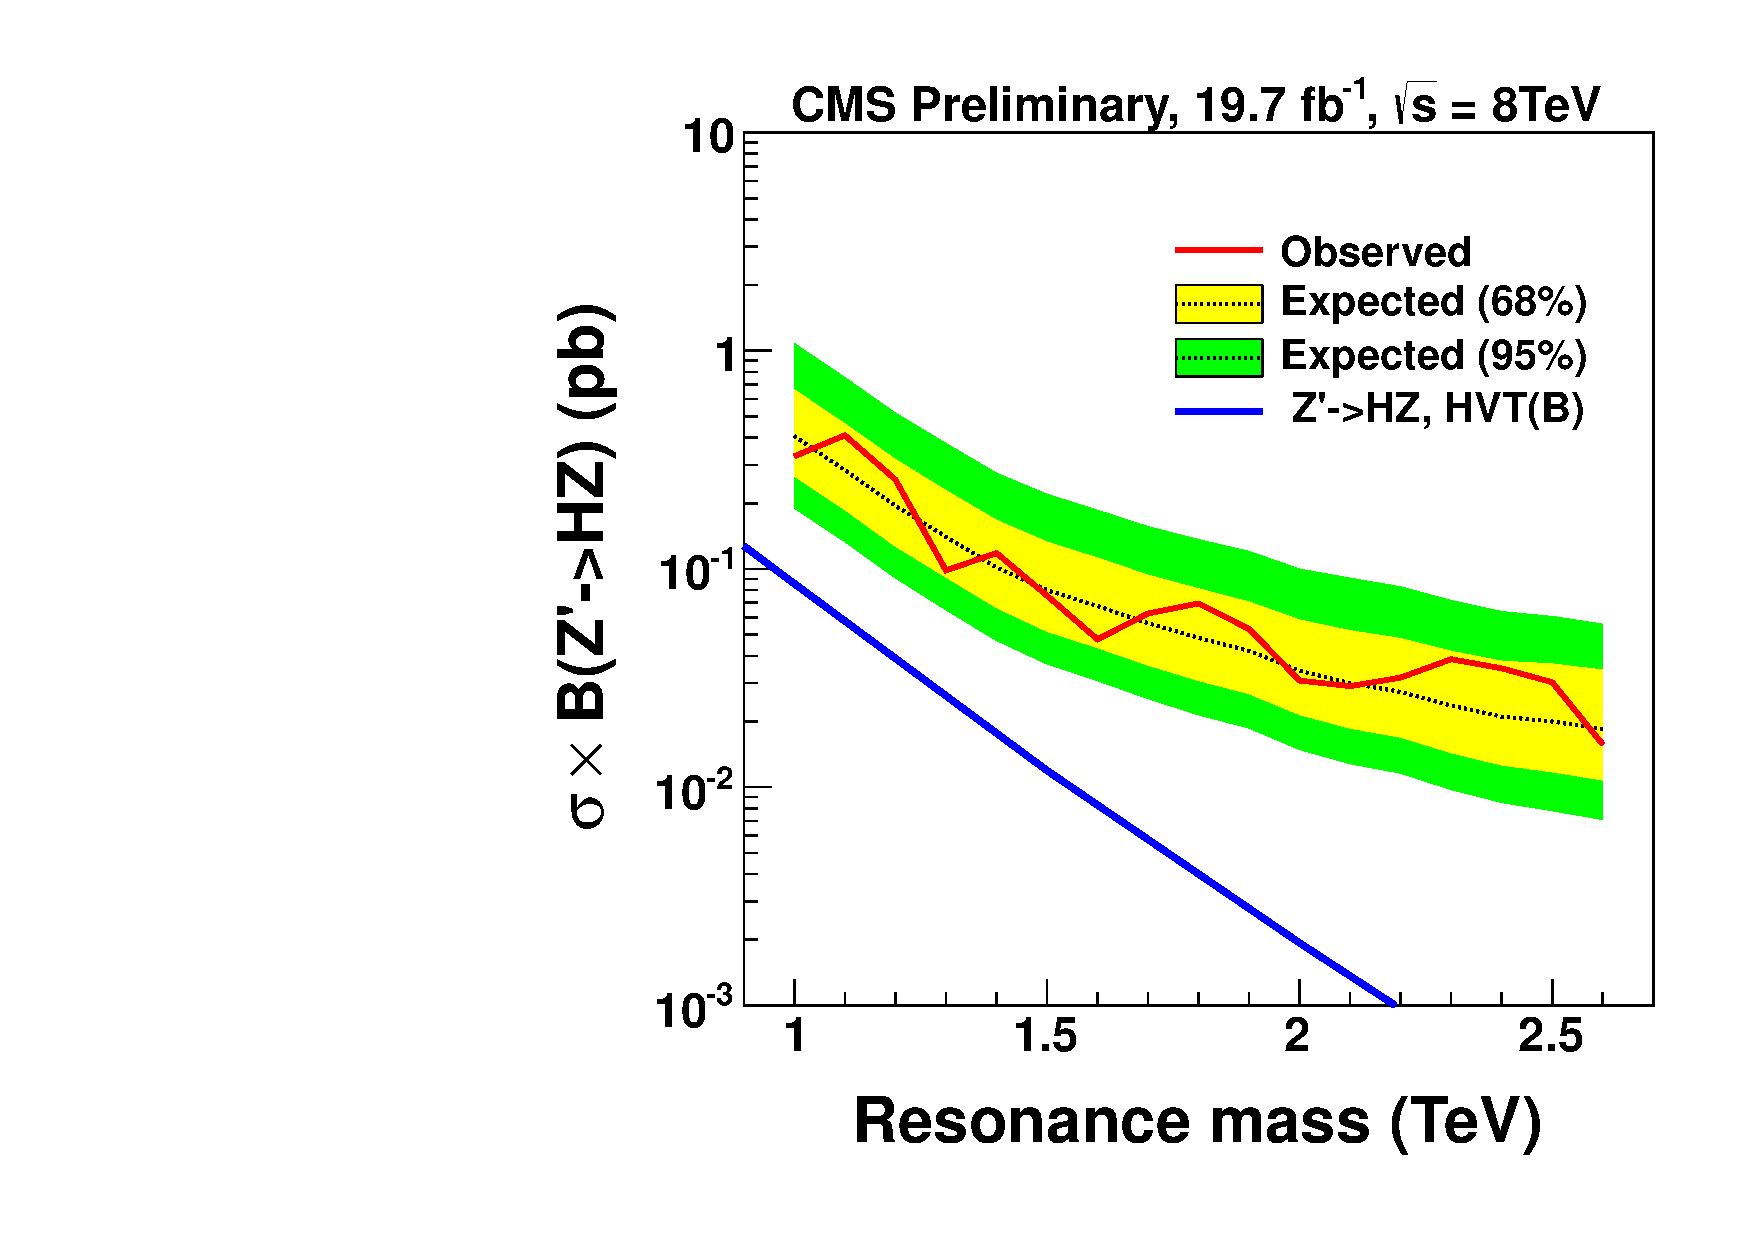
\includegraphics[width=0.49\textwidth]{brazilianFlag_HwwZqqHPLPHV.pdf}
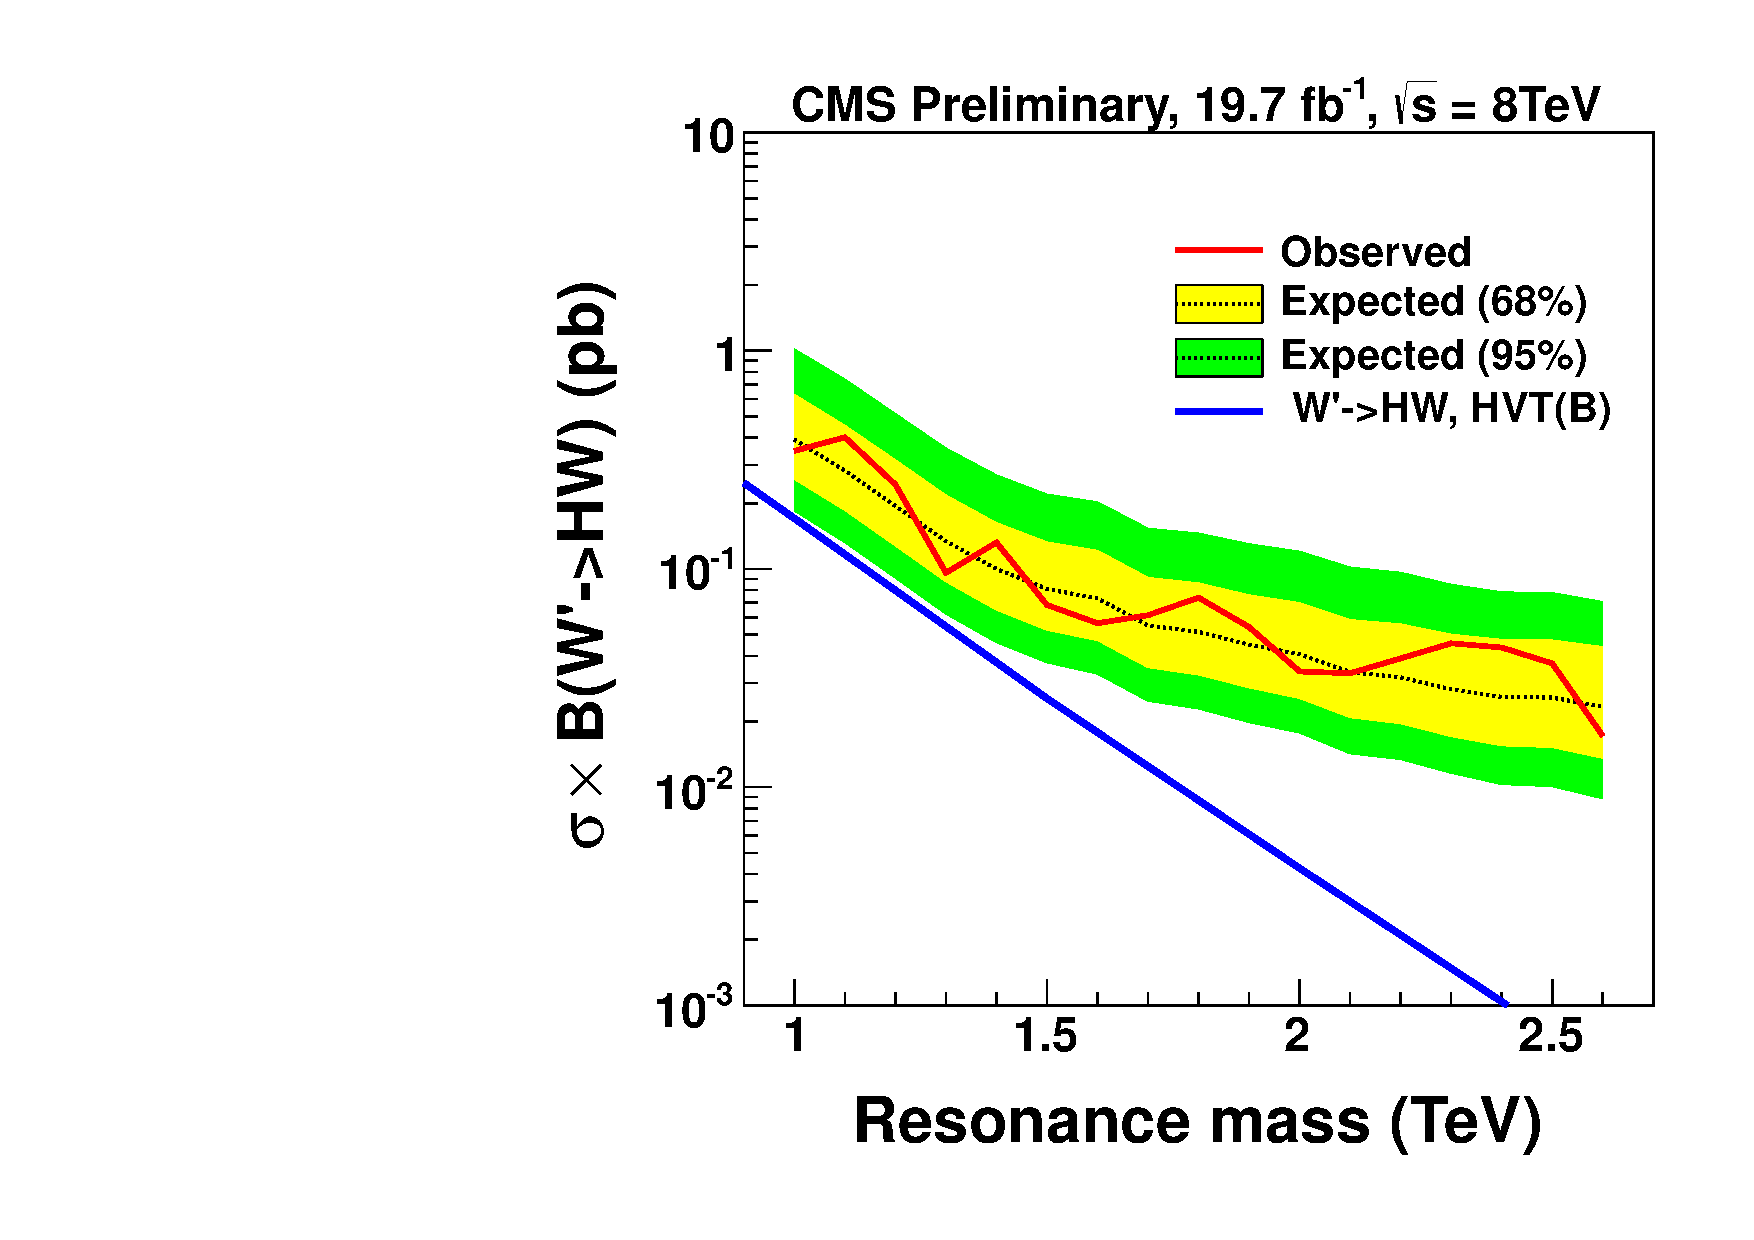
\includegraphics[width=0.49\textwidth]{brazilianFlag_HwwWqqHPLPHV.pdf}
\end{center}
\caption{Expected and observed limits for ${\rm Z'\to HZ}$(left) and ${\rm W' \to WZ}$(right)
 search for categories Hww1, Hww2 and Hww3. Branching ratios of $\Hww$, $\Hbb$ and V decays are
 taken into account. Theory model used here is HVT scenario B, arXiv:1402.4431.
% The high purity is on the bottom left. the low purity V-tagging on bottom right.
%  The predicted cross sections as a function of resonance mass for the considered benchmark models are overlaid.
}
\label{fig:HwwVCombined}
\end{figure*}




\clearpage
